Blockchain is a programmable, distributed ledger with an immutable history of transactions. 
For every transaction consensus has to be reached among the participating organisations (or commonly denoted as nodes) before it can be written on the ledger. %Examples of consensus protocols include Byzantine Fault Tolerance or Raft. 
Blockchain is programmable via the notion of a smart contract that is simply a piece of code, that is installed and executed within the Blockchain network; the execution of a smart contract's function creates a transaction. Note that the transaction is written on the ledger of each node concurrently. Consequently, the ledgers are always synchronised. If a node has some downtime, when it restarts, it automatically synchronises its ledger to the ledgers of the rest of the nodes. In addition, a single ledger (of a single node) cannot be tampered unless the attacker can manage to concurrently infiltrate at least the majority (if not all) of the nodes, depending on the consensus protocol used.

In the proposed architecture a blockchain network is created where every relevant organisation (e.g a hospital) participates. The user's permissions that control access for the SPHR are programmed using smart contracts. This allows versatility as the rules used to form the permissions can be updated whenever required. However, due to the Blockchain's nature, a single organisation cannot force an update of these rules as transactions will not be able to reach consensus and inevitably will not be written on the ledger.
The process flow for setting up access control is shown in Figure~\ref{fig:blockchain_flow} and described below.
\begin{enumerate}
    \item The Hospital (organisation) creates generic access rules about its data, these rules are implemented via smart contracts and written in the blockchain.
    \item The Patient creates access rules about this data, these rules are implemented via smart contracts and written in the blockchain.
    \item The patient's identifier is shared with the data requester (e.g. the doctor).
    \item The Doctor authenticates himself.
    \item The Doctor (individual, belonging to a group in an organisation) requests access to data about a patient (from a hospital). The doctor's identifier and the patient's identifier are checked against the access rules in the blockchain (check/audit trail).
    \item An access token is requested from the data vault to access the patient data.
    \item The data vault provides the access token.
    \item A response is sent to the doctor with the access token.
    \item The doctor requests data about the Patient to the data vault using the access token.
    \item The data vault provides the requested data.
\end{enumerate}

\begin{figure}[H]
    \centering
    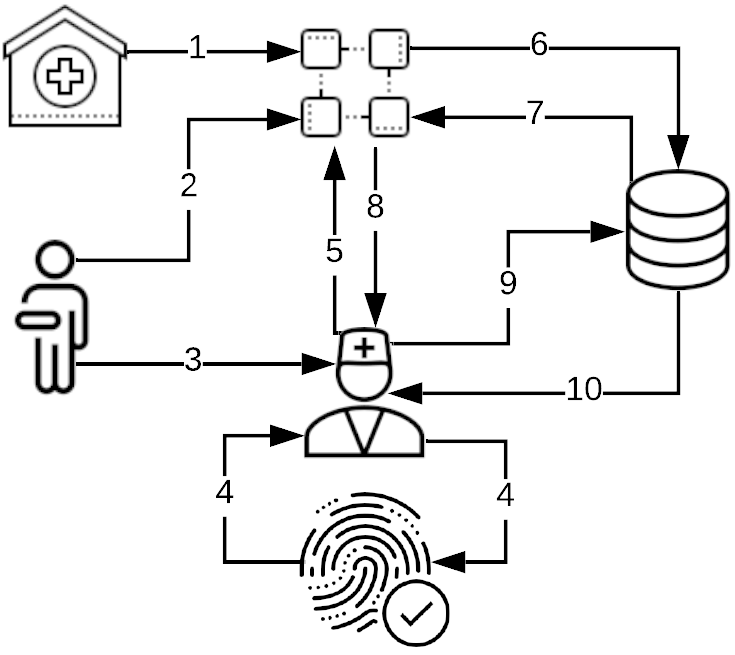
\includegraphics[width=70mm]{images/DataVault/blockchain.png}
    \caption{Process flow for access request}
    \label{fig:blockchain_flow}
\end{figure}
